
\documentclass[10pt]{article}

\usepackage{graphicx,amsmath,amssymb,subfigure,enumerate,versions}
\usepackage{multicol,multirow,mdframed}
\usepackage{epstopdf}
\usepackage{pstricks,auto-pst-pdf}
\usepackage{pst-all}
\usepackage{pst-ode}
\usepackage{pst-math}
\usepackage{hyperref}
\usepackage{listings}
%\usepackage{mcode}
\lstset{language=Matlab}
\DeclareGraphicsExtensions{.png,.jpg,.pdf}

% ************ Page Margins *************
\hoffset=-1.3in
\setlength{\textwidth}{7.5in}
%%%%% MARGINS
\topmargin 0pt
\advance \topmargin by -\headheight
\advance \topmargin by -\headsep
\textheight 9.5in

% ************ Shortcuts *************
\newcommand{\Z}{\mbox{\sf Z\hspace{-1.5mm}Z}}
\newcommand{\SolutionSeparator}{ \hfill \hfill \hrule \hfill \hfill }
\newcommand{\R}{\mbox{\rm I\hspace{-0.75mm}R}}
\columnsep=0.75in
\newcommand{\vsc}{\vspace{1mm}}
\newcommand{\D}{\Delta }
\newcommand{\ifd}{f(x)~dx}
\newcommand{\dd}{\frac{dy}{dx} \,} 
\newcommand{\der}[2]{\frac{d{#1}}{d{#2}} \,}
\newcommand{\ddx}[1]{\frac{d {#1}}{dx} \,} 
\newcommand{\ddy}[1]{\frac{d {#1}}{dy} \,} 
\newcommand{\ddz}[1]{\frac{d {#1}}{dz} \,} 
\newcommand{\ddt}[1]{\frac{d {#1}}{dt} \,} 
\newcommand{\ds}{\displaystyle } 
\newcommand{\la}{\lambda } 
\newcommand{\del}{\nabla } 
\newcommand{\zx}{\frac{\partial z}{\partial x} \,}
\newcommand{\zy}{\frac{\partial z}{\partial y} \,}
\newcommand{\dx}{\frac{\partial f}{\partial x} \,}
\newcommand{\dy}{\frac{\partial f}{\partial y} \,}
\newcommand{\pp}[2]{\frac{\partial {#1}}{\partial {#2}} \,}
\newcommand{\ppx}{\frac{\partial }{\partial x} \,}
\newcommand{\ppy}{\frac{\partial }{\partial y} \,}
\renewcommand{\thesection}{\Roman{section}}
\newcommand{\vi}{\vec{i}}
\newcommand{\vj}{\vec{j}}
\newcommand{\vk}{\vec{k}}
\newcommand{\vv}{\vec{v}}
\newcommand{\lan}{\left\langle}
\newcommand{\ran}{\right\rangle}
\newcommand{\degr}{^{\circ}}

% *** Define the printed question style ***
\newcommand{\q}[1]{ {\em #1} }
% \renewcommand{\q}[1]{ {} }

\newcommand{\notice}{ \begin{center}Some problems and solutions
    selected or adapted from \\ Stewart {\em Calculus-Early
      Transcendentals} and Hughes-Hallett {\em Calculus} .\end{center}
}

% *** Overwrite, if desired, the question format
\includeversion{Question} 
\includeversion{Solution}

\newcommand{\multicolstart}{ }
\newcommand{\multicolend}{ }

\renewenvironment{Question}
{ \begin{mdframed}[nobreak=true,hidealllines=true,backgroundcolor=gray!50,innerleftmargin=5ex] }
{ \end{mdframed} }


% *** Footnoting with symbols ***
\long\def\symbolfootnote[#1]#2{\begingroup%
\def\thefootnote{\fnsymbol{footnote}}\footnote[#1]{#2}\endgroup}

\newcommand{\WeekTitleOne}{Derivatives - Foundations}
\newcommand{\WeekTitleTwo}{Derivatives - Linearization and Applications}
\newcommand{\WeekTitleThree}{Derivatives - Modeling}
\newcommand{\WeekTitleFour}{Integrals - Foundations}
\newcommand{\WeekTitleFive}{Integrals - Techniques}
\newcommand{\WeekTitleSix}{Integrals - Modeling}
\newcommand{\WeekTitleSeven}{Differential Equations - }
\newcommand{\WeekTitleEight}{Differential Equations - }
\newcommand{\WeekTitleNine}{Differential Equations - }
\newcommand{\WeekTitleTen}{Linear Algebra - }
\newcommand{\WeekTitleEleven}{Linear Algebra - }
\newcommand{\WeekTitleTwelve}{Linear Algebra - }


\begin{document}


\begin{center}
\subsection*{Week \#2 - \WeekTitleTwo}
\end{center}


\subsection*{Linear Approximations and Tangent Lines}
\begin{enumerate}[1.]
\begin{multicols}{2}

  % ***************************************************************
\item
  \begin{Question}
    Find the equation of the tangent line to the graph of $f$ at
    (1,1), where $f$ is given by $f(x) = 2x^3 - 2x^2 + 1$.
  \end{Question}
  \begin{Solution}
    $f(x) = 2x^3 - 2x^2 + 1$.  \\
    In general, the slopes of the function are given by $f'(x) = 6x^2
    -
    4x$ \\
    At the point $(1,1)$ (which you should check is actually on the graph of $f(x)$!), the slope is \\
    $f'(1) = 6 - 4 = 2$ \\
    Using the point/slope formula for a line (or the tangent line
    formula), a line tangent to the graph of $f(x)$ at the point
    $(1,1)$ is
    \begin{align*} y & = f'(1) (x-1) + f(1)\\
      & = 2 (x-1) + 1 \\
      \mbox{ or } y & = 2x - 1
    \end{align*}
    
  \end{Solution}
  % ***************************************************************
\item
  \begin{Question}
    \begin{enumerate}[(a)]
    \item Find the equation of the tangent line to $f(x) = x^3$ at
      $x=2$.
    \item Sketch the curve and the tangent line on the same axes, and
      decide whether using the tangent line to approximate $f(x) =
      x^3$ would produce {\em over-} or {\em under-}estimates of
      $f(x)$ near $x=2$.
    \end{enumerate}
    
  \end{Question}
  \begin{Solution}
    \begin{enumerate}[(a)]
    \item $f(x) = x^3$, so $f'(x) = 3x^2$.  \\
      At $x=2$, $f(2) = 8$ and $f'(2) = 12$, so the tangent line to
      $f(x)$ at $x=2$ is
$$ y = 12 (x-2) + 8$$ 
\item ~ \\
  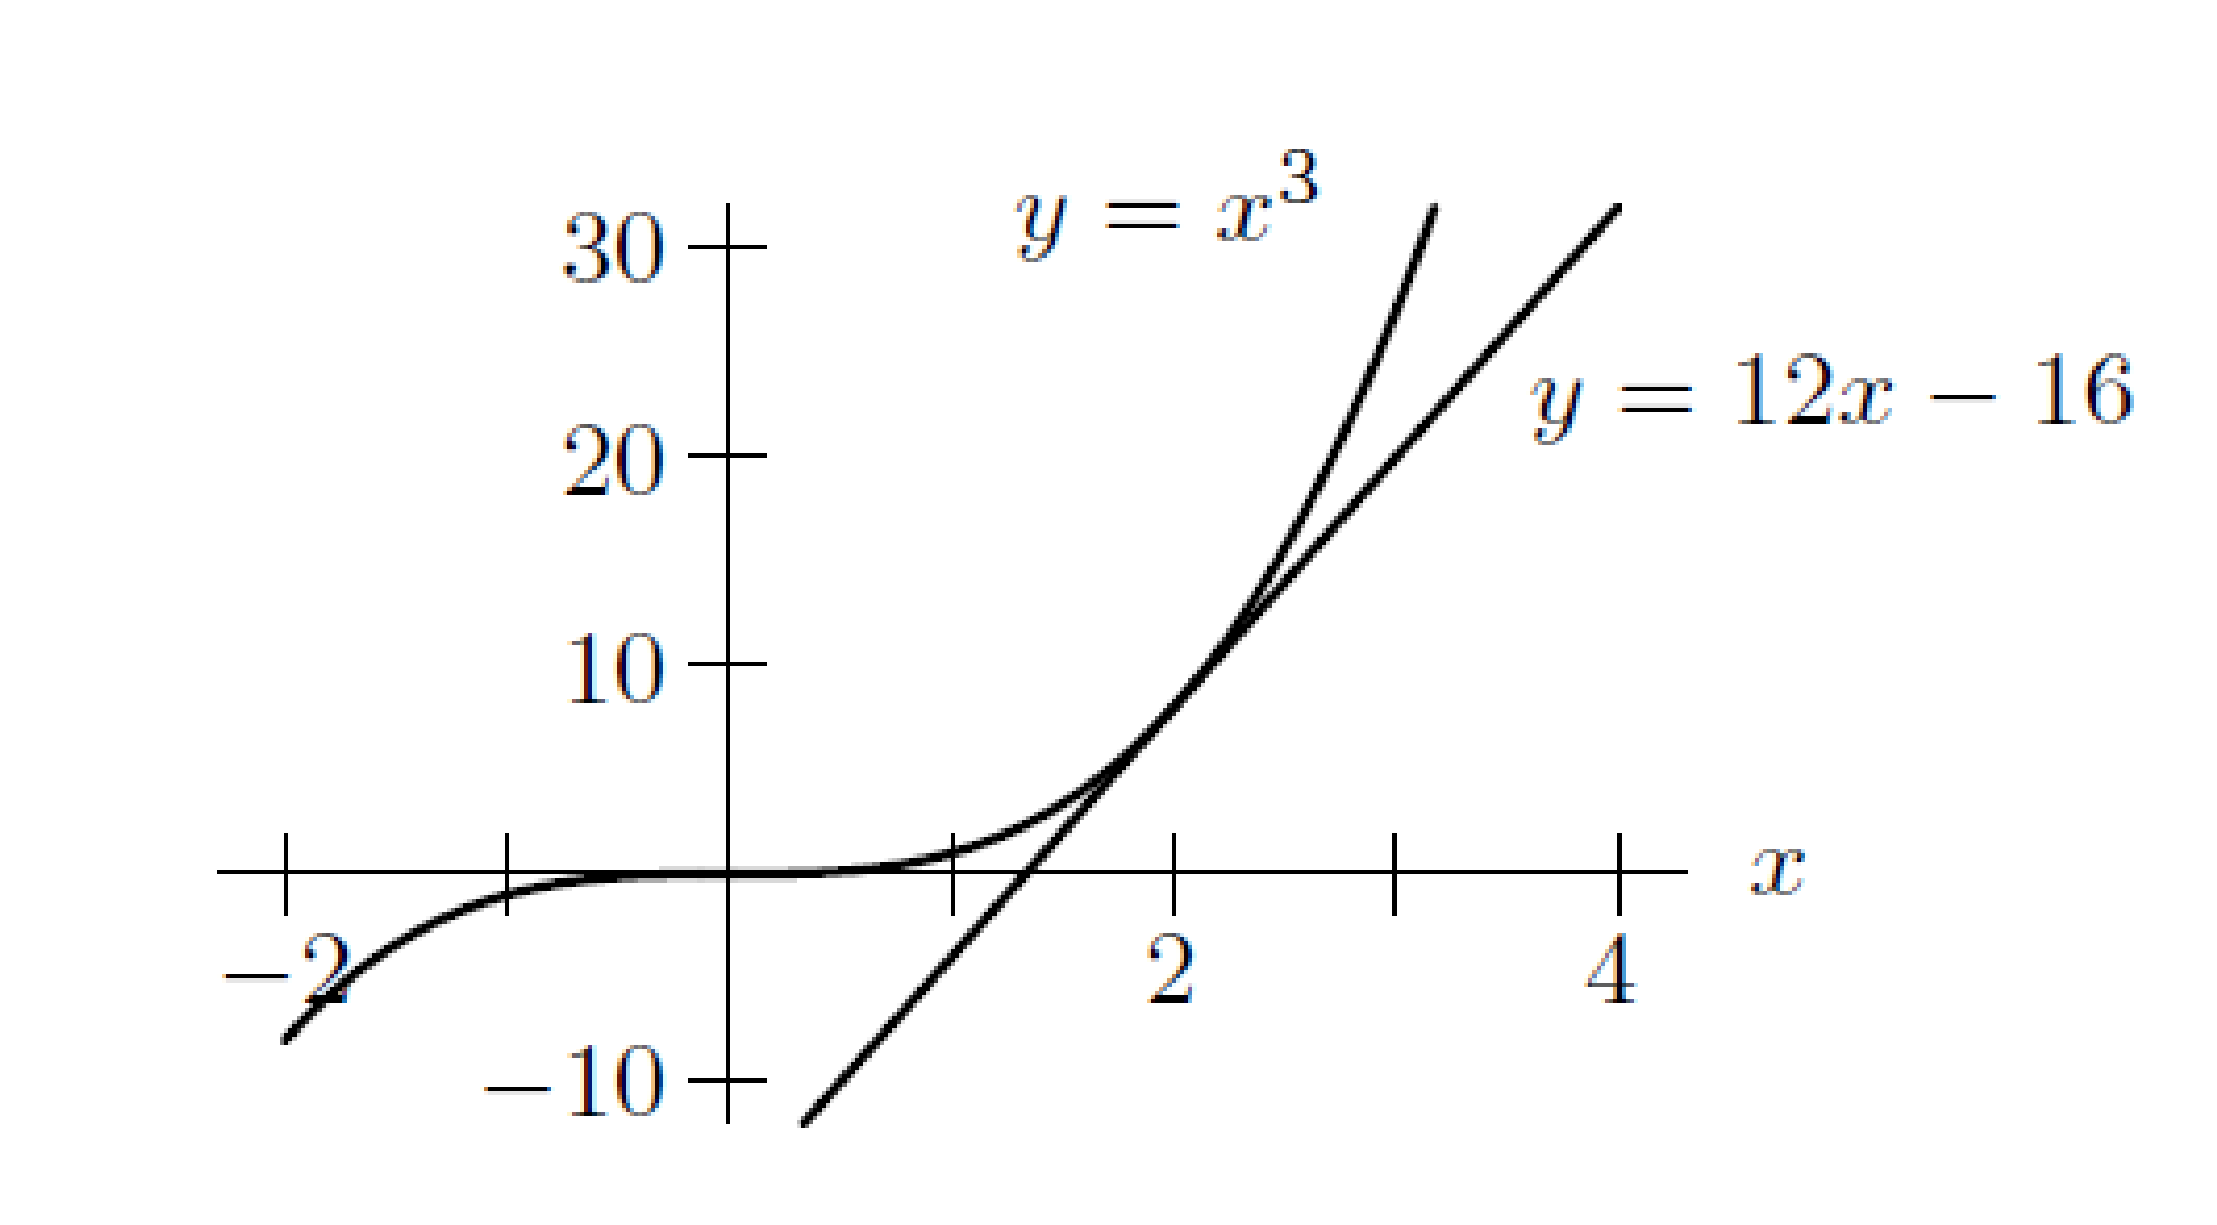
\includegraphics[width=2.0in]{graphics/Week02_TangentLines/Tangent_x_cubed} \\
  From the graph of $y =x^3$, it is clear that the tangent line at
  $x=2$ will lie {\em below} the actual curve. This means that using
  the tangent line to estimate $f(x)$ values will produce {\em
    underestimates} of $f(x)$.
\end{enumerate}
    
\end{Solution}
% ***************************************************************
\item
  \begin{Question}
    Find the equation of the line tangent to the graph of \(f\) at
    \((3,57)\), where \(f\) is given by \(f(x)= 4 x^3 - 7 x^2 + 12\).
    \par \end{Question}
  \begin{Solution}
    Differentiating gives \(f'(x) = 12 x^2 - 14 x\), so \(f'(3) =
    66\).  Thus the equation of the tangent line is \(y - 57 = 66 ( x
    - 3 )\), or \(y = 57 + 66 (x - 3 )\).
    \par\end{Solution}
  % ***************************************************************
\item
  \begin{Question}
    Given a power function of the form \(f(x)=ax^n\), with \(f'(3) =
    16\) and \(f'(6) = 128\), find \(n\) and \(a\).
    \par
    \par \end{Question}
  \begin{Solution}
 
    Since \(f(x)=ax^n\), \(f'(x)=anx^{n-1}\).  We know that
    \(f'(3)=(an)3^{n-1} = 16\), and \(f'(6) = (an) 6^{n-1} = 128\).
    Therefore,
    \[\frac{f'(6)}{f'(3)} = \frac{128}{16} = 8.\]
    But
    \[\frac{f'(6)}{f'(3)} = \frac{(an)6^{n-1}}{(an)3^{n-1}} =
    2^{n-1},\] so \(2^{n-1} = 8\), and so \(n = 4\).
    \par
    Substituting \(n=4\) into the expression for \(f'(3)\), we get \(4
    a 3^{3} = 16\), so \(a = \frac{4}{27}\).
    \par\end{Solution}
  % ***************************************************************
\item
  \begin{Question}
    Find the equation of the line tangent to the graph of \(f\) at
    \((2,1)\), where \(f\) is given by \(f(x)= 2 x^3 - 5 x^2 + 5\).
    \par \end{Question}
  \begin{Solution}
 
    Differentiating gives \(f'(x) = 6 x^2 - 10 x\), so \(f'(2) = 4\).
    Thus the equation of the tangent line is \(y - 1 = 4 ( x - 2 )\),
    or \(y = 1 + 4 (x - 2 )\).
    \par\end{Solution}

  % *******************************
\item
  \begin{Question}
 
\par 
Find all values of \(x\) where the tangent lines to \(y=x^{8}\) and
\(y=x^{9}\) are parallel.
\par \end{Question}
\begin{Solution}
 
  Let \(f(x)=x^{8}\) and let \(g(x)=x^{9}\). The two graphs have
  parallel tangent lines at all \(x\) where \(f'(x)=g'(x)\).
  \[f'(x) = g'(x)\]
  \[8x^{7} = 9x^{8}\]
  \[8x^{7}-9x^{8} = 0\]
  \[x^{7}\!\left(8-9x\right) = 0\] hence, \(x=0\) or
  \(x=\frac{8}{9}\).

  The point at $x=0$ is easy to visualize (both graphs are flat
  there).  Here is a graph showing the parallel tangents at $x=8/9$.

  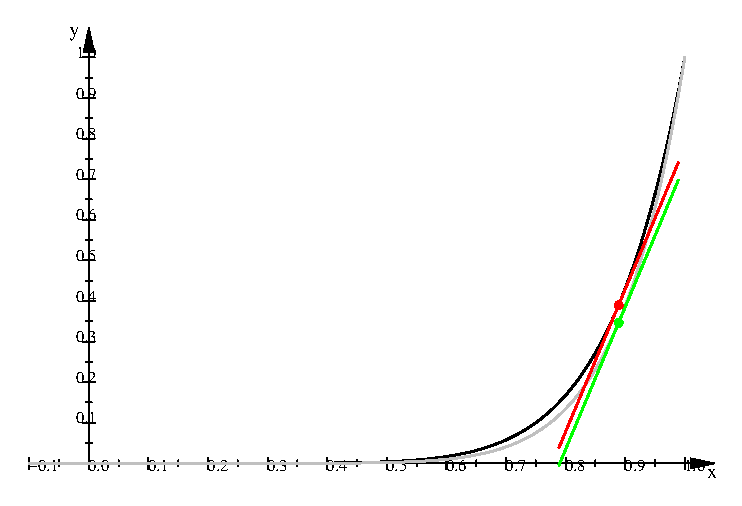
\includegraphics[width=0.8\linewidth]{graphics/Week02_TangentLines/TangentTo_x8_x9}
  \par\end{Solution}
% ***************************************************************
\item
  \begin{Question}
    Consider the function \(f(x)=9-e^x\).
    \begin{enumerate}[(a)]
    \item Find the slope of the graph of \(f(x)\) at the point where
      the graph crosses the \(x\)-axis.
      \par
    \item

      Find the equation of the tangent line to the curve at this
      point.
      \par
    \item Find the equation of the line perpendicular to the tangent
      line at this point. (This is the {\it normal} line.)
    \end{enumerate}
    \par \end{Question}
  \begin{Solution}
    \begin{enumerate}[(a)]
    \item \(f(x) = 9-e^x\) crosses the \(x\)-axis where \(0 = 9
      -e^x\), which happens when \(e^x = 9\), so \(x = \ln 9\).  Since
      \(f'(x) = -e^{x}\), \(f'(\ln 9) = -9\).
      \par
    \item \(y = -9 ( x - \ln(9) )\).
      \par
    \item The slope of the normal line is the negative reciprocal of
      the slope of the tangent, so \(y = \frac{1}{9} (x - \ln(9))\).
    \end{enumerate}
    \par\end{Solution}
  % ***************************************************************
\item
  \begin{Question}
    Consider the function $y = 2^x$.
    \begin{enumerate}[(a)]
    \item Find the tangent line based at $x=1$, and find where the
      tangent line will intersect the $x$ axis.
    \item Find the point on the graph $x=a$ where the tangent line
      will pass through the origin.
    \end{enumerate}
  \end{Question}
  \begin{Solution}
    \begin{enumerate}[(a)]
    \item  We find the linearization using $f(x) = 2^x$, so
$f'(x) = 2^x \ln(2)$ (non-$e$ exponential derivative rule).

At the point $x=1$, $f(1) = 2^1 = 2$ and $f'(1) = 2^1 \ln(2)$, so the linear approximation to $f(x)$ is 

$L(x) = 2+(2 \ln(2))(x-1)$. 

Solving for where this line intersects the $x$ axis (or the $y=0$
line), we find the $x$ intercept is approximately -0.4427.

\item This question is more general.  Instead of asking for a
  linearization at a specific point, it is asking ``at what point
  would the linearization pass through the origin?''  Let us give the
  point a name: $x=a$ (as opposed to $x=1$ used in part (a)).

From the function and the derivatives, the linearization at the point $x=a$ is given by:
$$L_a(x) = \underbrace{2^a}_{f(a)} + \underbrace{2^a \ln(2)}_{f'(a)}(x-a)$$

That is true in general, but we want the point $x=a$ where the
linearization will go through $(0,0)$, i.e. for which $L_a(0) = 0$:
\begin{align*}
0 & = 2^a + 2^a \ln(2) (0-a)  \\
\mbox{ Solving for }a,~~~~~ 0 & = 2^a (1 - a \ln(2)) \\
0 & = 1 - a \ln(2) \\
a \ln(2)  & = 1  \\
a & = \frac{1}{\ln(2)} \approx 1.442  \\
\end{align*}
At that $x$ point, the graph of $y = 2^x$'s tangent line will pass
exactly through the origin.
    \end{enumerate}
  \end{Solution}

  % ***************************************************************
\item
  \begin{Question}
    \begin{enumerate}[(a)]
    \item Find the tangent line approximation to $f(x) = e^x$ at
      $x=0$.
    \item Use a sketch of $f(x)$ and the tangent line to determine
      whether the tangent line produces over- or under-estimates of
      $f(x)$.
    \item Use your answer from part (b) to decide whether the
      statement $e^x \ge 1 + x$ is always true or not.
    \end{enumerate}
  \end{Question}
  \begin{Solution}
    \begin{enumerate}[(a)]
    \item $f(x) = e^x$, so $f'(x) = e^x$ as well.\\
To build the tangent line at $x=0$, we use $a=0$ as our reference point:
$f(0) = e^0 = 1$, and $f'(0) = e^0 = 1$.
The tangent line is therefore \\
$l(x) = 1 (x-0) + 1 = x + 1$
\item  ~ \\
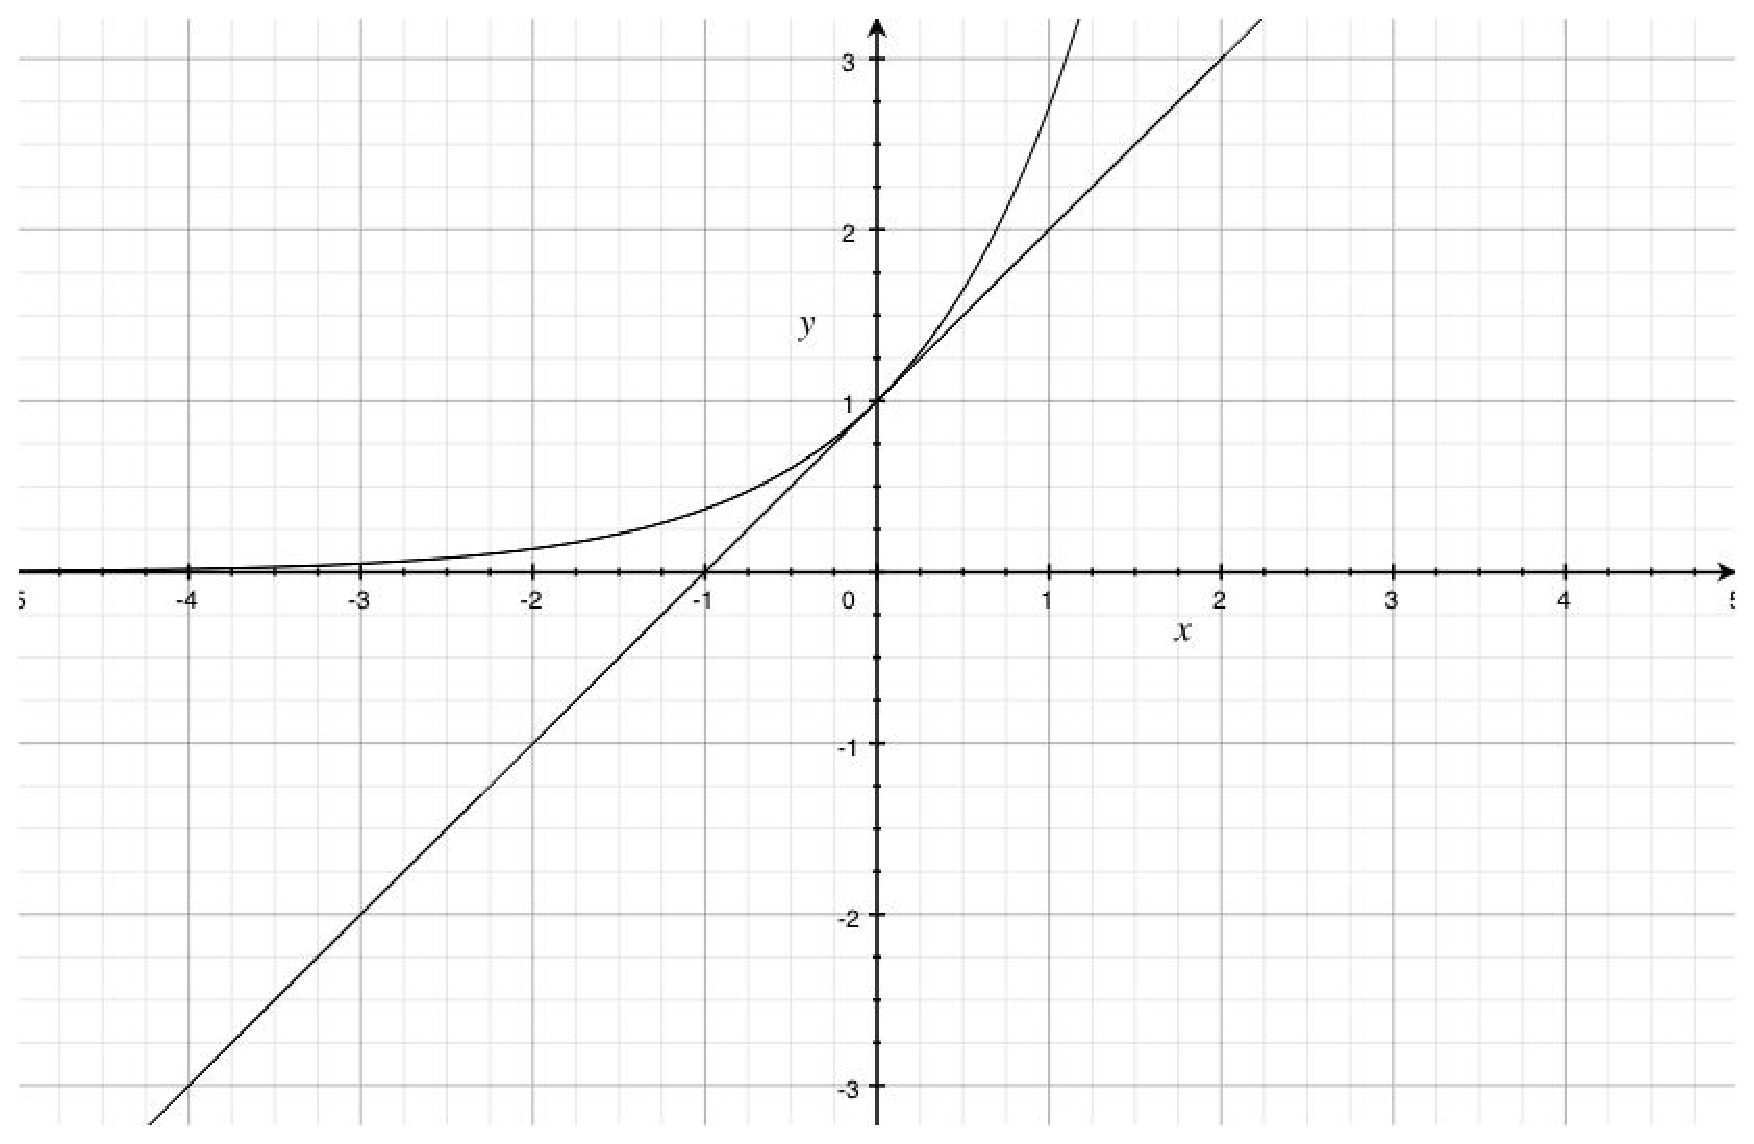
\includegraphics[width=0.8\linewidth]{graphics/Week02_TangentLines/exp_tangent}

Since the exponential graph is concave up, it curves upwards away from
the graph.  This means that the linear approximation will always be an
under-estimate of the original function.
\item Since the linear function will always underestimate the value of $e^x$, we can
conclude that
$$1+x \le e^x$$, and they will be equal only at the tangent point, $x=0$.
\end{enumerate}
    
  \end{Solution}

  % ***************************************************************
\item
  \begin{Question}
   The speed of sound in dry air is
$$f(T) = 331.3 \sqrt{1 + \frac{T}{273.15}} \mbox{m/s} $$
where $T$ is the temperature in degrees Celsius.  Find a linear
function that approximates the speed of sound for temperatures near
$0^o$ C.
  \end{Question}
  \begin{Solution}
    
  \begin{align*}
    f(T) & = 331.3 \sqrt{1 + \frac{T}{273.15}} \\
 f'(T) & = 331.3 \left(\frac{1}{2}\right) \left(\frac{1}{\sqrt{1 + \frac{T}{273.15}}}\right) \frac{1}{273.15} 
\end{align*}
  \begin{align*}
    \mbox{ so at } T = 0^o \mbox{ C}, ~~~ f(0) & = 331.3 & f'(0) & =
    \frac{331.3}{(2)(273.15)} \approx 0.606
  \end{align*}
  Thus the speed of sound for air temperatures around $0^o$ C is
$$f(T) \approx 0.606 (T - 0) + 331.3, \mbox{ or } f(t) \approx 0.606 T + 331.3 \mbox{ m/s}$$

  \end{Solution}
  % ***************************************************************
\item
  \begin{Question}
    Find the equations of the tangent lines to the graph of $y =
    \sin(x)$ at $x=0$, and at $x=\pi/3$. 
    \begin{enumerate}
    \item Use each tangent line to approximate $\sin(\pi/6)$. 
    \item Would you expect these results to be equally accurate, given
      that they are taken at equal distances on either side of
      $\pi/6$?  If there is a difference in accuracy, can you explain
      it?
    \end{enumerate}
 
  \end{Question}
  \begin{Solution}
    \begin{enumerate}[(a)]
  \item At $x=0$, the tangent line is defined by 
$f(0) = 0$ and $f'(0) = 1$, so 
$$y = 1(x-0) + 0 = x$$
is the tangent line to $f(x)$ at $\ds x=\frac{\pi}{3}$.

  At $\ds x=\frac{\pi}{3}$, the tangent line is defined by 
$(\pi/3) = \frac{\sqrt{3}}{2}$ and $f'(\pi/3) = \frac{1}{2}$, so 
$$y = \frac{1}{2}\left(x-\frac{\pi}{3}\right) + \frac{\sqrt{3}}{2}$$
is the tangent line to $f(x)$ at $x=0$.

The estimates of each tangent line at the point $x=\pi/6$ would be
\begin{itemize}
\item Based on $x=0$ tangent line, $f(x) \approx x$, so $f(\pi/6) \approx
  \pi/6 \approx 0.5236 $.
\item Based on $x=\pi/3$ tangent line,
$\ds f(x) \approx  \frac{1}{2}\left(x-\frac{\pi}{3}\right) + \frac{\sqrt{3}}{2}$, \\
so 
$\ds f(\pi/6) \approx  \frac{1}{2}\left(\pi/6-\frac{\pi}{3}\right) + \frac{\sqrt{3}}{2} \approx 0.6042 $
\item The {\bf actual} value of $f(x) = \sin(x)$ at $x= \pi/6$ is
  $\sin(\pi/6) = 0.5$. 
\end{itemize}
\item From these calculations, the estimate obtained by using the
  tangent line based at $x=0$ gives the more accurate prediction for
  $f(x)$ at $x=\pi/6$

A sketch might help explain these results.

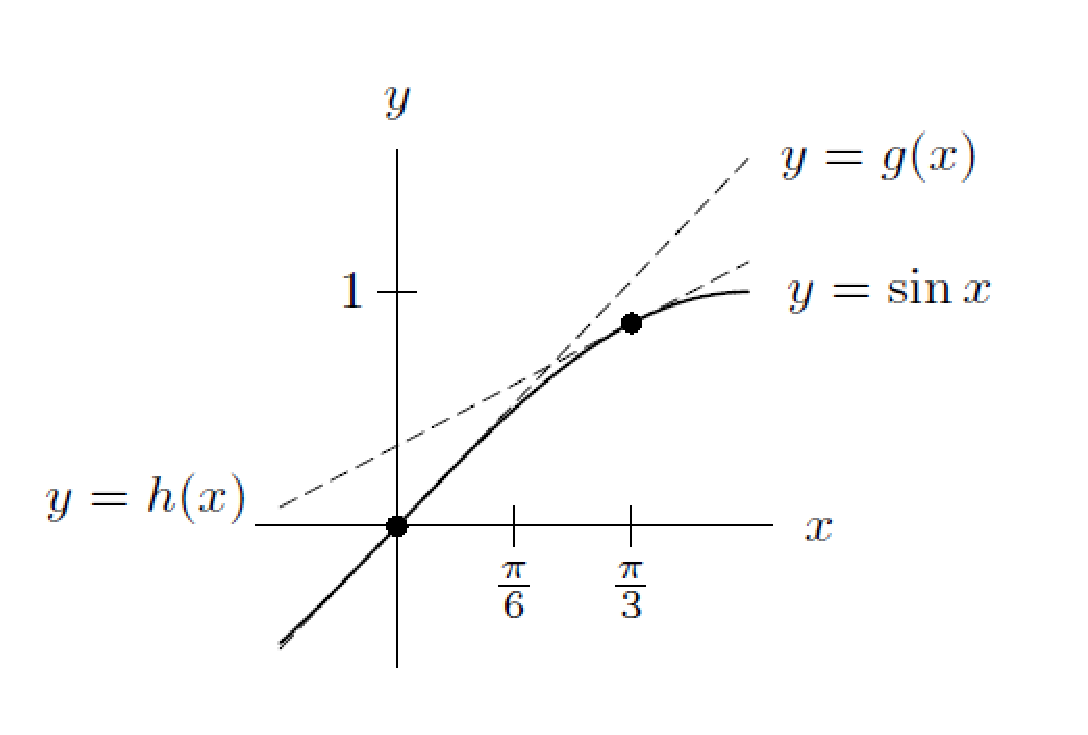
\includegraphics[width=0.8\linewidth]{graphics/Week02_TangentLines/Sine_tangents}

In the interval $x \in [0, \pi/6]$, the function stays very close to
linear (i.e. does not curve much), which means that the tangent
line stays a good approximation for a relatively long time.

The function is most curved/least linear around its peak, so the
linear approximation around $x = \pi/3$ is less accurate even over the
same $\Delta x$.
    \end{enumerate}

  \end{Solution}


%   % ***************************************************************
% \item
%   \begin{Question}
%     Find the {\bf quadratic} polynomial $g(x) = ax^2 + bx + c$ which
%     best fits the function $f(x) = e^x$ at $x=0$, in the sense that
% $$ g(0) = f(0), g'(0) = f'(0), \mbox{ and  } g''(0) = f''(0)$$
% \end{Question}
% \begin{Solution}
% \begin{align*}
% f(x) & = e^x \\
% \mbox{ so } f'(x) = e^x \\
% \mbox{ and } f''(x) = e^x \\
% \mbox{Evaluating at $x=0$,} \\
% f(0) = f'(0) = f''(0) & = 1 \\
%   \end{align*}
% Comparing with the derivatives of the quadratic,
% \begin{align*}
% g(x) & = ax^2 + bx + c \\
% \mbox{ so } g'(x) = 2ax + b \\
% \mbox{ and } g''(x) = 2a \\
% \mbox{Evaluating at $x=0$,} \\
% g(0) = c, g'(0) = b, & \mbox{ and } g''(0) = 2a
%   \end{align*}
%   For $g(x)$ to fit the shape of $f(x)$ near $x=0$, we would then pick
%   $c = 1$, $b = 1$ and $2a= 1$ or $a= 0.5$, so
% $$ g(x) = 0.5 x^2 + x + 1$$
% would be the best fit quadratic to $f(x) = e^x$ near $x=0$.

% Here is a graph of the two functions, $f(x) = e^x$ in black, $g(x) = 0.5 x^2 + x + 1$ in red.  
% Notice how similar they look near their intersection.

% 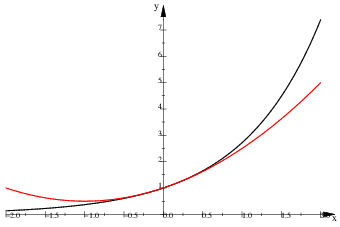
\includegraphics[width=0.8\linewidth]{graphics/Week02_TangentLines/Exp_quadratic_fit}
    
% \end{Solution}

% ***************************************************************
\item
  \begin{Question}
    Consider the graphs of $y = \sin(x)$ (regular sine graph), and $y
    = k e^{-x}$ (exponential decay, but scaled vertically by $k$).

    If $k \ge 1$, the two graphs will intersect.  What is the smallest
    value of $k$ for which two graphs will be {\em tangent} at that
    intersection point?

    
  \end{Question}
  \begin{Solution}
Let $f(x) = \sin(x)$ and $g(x) = k e^{-x}$.  They intersect
  when $f(x) = g(x)$, and they are tangent at that intersection if
  $f'(x) = g'(x)$ as well.  Thus we must have
  \begin{align*}
    \sin(x) & = k e^{-x} & \mbox{ and } \cos(x) & = -k e^{-x}
  \end{align*}
  We can't solve either equation on its own, but we can divide one by
  the other:
  \begin{align*}
    \frac{\sin(x)}{\cos(x)} & = \frac{k e^{-x}}{-ke^{-x}} \\
    \tan(x) & = -1 \\
    x & = \frac{3\pi }{4}, \frac{7 \pi}{4}, \ldots \\
  \end{align*}
  Since we only need one value of $k$, we try the first value, $x = 3
  \pi/4$.
\begin{align*}
\sin(3\pi/4) & = k e^{-3\pi/4} \\
\frac{1}{\sqrt{2}} e^{3\pi/4} & = k  \\
k & \approx 7.46 
\end{align*}
We confirm our answer by verifying both the values and derivatives are
equal at $x = 3\pi/4$,
  \begin{align*}
    \sin(3 \pi / 4) & = 7.46 e^{-3\pi/4} \approx 0.7071  \mbox{ (same $y$: intersection)}\\
 \mbox{ and } \cos(3\pi/4) & = -7.46 e^{-3\pi/4} \approx -0.7071  \mbox{ (same derivative)}
  \end{align*}

  The actual point of tangency is at $\ds (x, y) = \left(\frac{3\pi}{4},
    \frac{1}{\sqrt{2}}\right)$.  A sketch is shown below.
  
  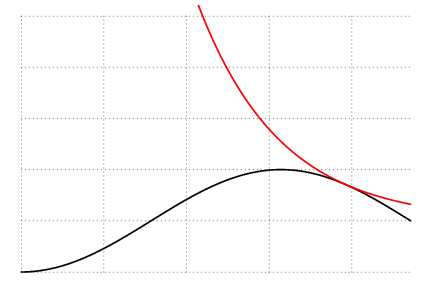
\includegraphics[width=0.8\linewidth]{graphics/Week02_TangentLines/Sine_exp_tangency} 
    
  \end{Solution}
  % ***************************************************************
\item
  \begin{Question}
    \begin{enumerate}[(a)]
    \item Show that $1 + kx$ is the local linearization of $(1+x)^k$ near $x=0$.
    \item Someone claims that the square root of 1.1 is about 1.05.
      Without using a calculator, is this estimate about right, and
      how can you decide using part (a)?
    \end{enumerate}
    
  \end{Question}
  \begin{Solution}
  \begin{enumerate}[(a)]
    \item\begin{align*}
       f(x) & = (1 + x)^k & f'(x) & = k (1+x)^{k-1}   \\
\mbox{ so at } x = 0, ~~~ f(0) & = 1^k = 1 & f'(0) &= k (1^{k-1}) = k\\
  \end{align*}
so the tangent line at $x=0$ will be 
$$y = k (x-0) + 1 \mbox{ or } y = 1 + kx$$
\item As an estimate for the square root of $1.1$, we could note that
  $\sqrt{1.1} = (1 + 0.1)^{1/2}$. This matches exactly the form of
  $f(0.1)$ if we choose $k = \frac{1}{2}$. From our linearization
  above,
$$f(0.1) \approx 1 + \frac{1}{2}(0.1) = 1.05$$
so yes, a good approximation for $\sqrt{1.1}$ is 1.05.  (Calculator
gives the value of $\approx 1.0488$.
  \end{enumerate}
  \end{Solution}

  % ***************************************************************
\item
  \begin{Question}
    \begin{enumerate}
    \item Find the local linearlization of $e^x$ near $x=0$. 
    \item Square your answer to part (a) to find an approximation to
      $e^{2x}$.
    \item Compare your answer in part (b) to the actual linearization
      to $e^{2x}$ near $x=0$, and discuss which is more accurate.
    \end{enumerate}
  \end{Question}
  \begin{Solution}
    \begin{enumerate}[(a)]
    \item $e^x$ has a tangent line/local linearization near $x=0$ of
      $y = x + 1$ (slope 1, point (0, 1)).

    \item Multiplying this approximation by itself, we get
      $(e^x)(e^x)$ or $e^{2x} \approx (x+1)(x+1) = x^2 + 2x + 1$

    \item To compare with the actual linearization of $g(x) = e^{2x}$,
      we find its derivative and value at $x=0$,
  \begin{align*}
    g(x) & = e^{2x} & g(0) & = 1 \\
g'(x) & = 2 e^{2x} & g'(0) & = 2 \\
  \end{align*}
  so a linearization of $g(x) = e^{2x}$ near $x=0$ is $y = 2 (x-0) + 1$ or 
$$ y = 2x + 1$$
Note that his is the same as the approximation we obtained before,
except that our product version had an additional term, $x^2$.

These approximations give the same straight-line estimate of the
function, but I would expect the first (multiplication) version to be
more accurate because it contains more information (the squared term
that the pure linear approximation was missing).

We will see more of this idea in Taylor polynomials and Taylor series.
    \end{enumerate}
  \end{Solution}
  % ***************************************************************
\item
  \begin{Question}
    \begin{enumerate}
    \item Show that $1-x$ is the local linearization of $\ds
      \frac{1}{1+x}$ near $x=0$.
    \item From your answer to part (a), show that near $x=0$, 
      $$\frac{1}{1+x^2} \approx 1-x^2.$$
    \item Without differentiating, what do you think the derivative of
      $\ds \frac{1}{1+x^2}$ is at $x=0$?
    \end{enumerate}

    
  \end{Question}
  \begin{Solution}
    
  \begin{enumerate}[(a)]
  \item Let $f(x) = 1/(1+x)$.  Then $f'(x) = \frac{-1}{(1+x)^2}$. \\
    At $x=0$, $f(0) = 1$ and $f'(0) = -1$. \\
    So near $x=0$, $f(x) \approx -1 x + 1 = -x + 1$ \\
  \item For small $x$ values (i.e. $x$ near zero), we can approximate
    $1/(1+x)$ with $1-x$.  Replace the variable $x$ with $y$ (because
    the name doesn't matter),
$$1/(1+y)  \approx 1-y$$
If we choose $y$ small but equal to $x^2$, then 
$$\frac{1}{1 + x^2} \approx 1-x^2$$
\item The linearization of $1/(1+x^2)$ is the linear part of $1 -
  x^2$, or just $1$.  Since the derivative at $x=0$ is the coefficient
  for $x$ in the linear part, this means $\ds \ddx ~\frac{1}{1+x^2}$ at $x=0$
  must equal zero.
\end{enumerate}
  \end{Solution}
  % ***************************************************************
% \item
%   \begin{Question}
%     \begin{enumerate}[(a)]
%     \item Find the local linearization of

%       \[f(x) = \frac{1}{1 + 2 x}\] near \(x = 0\).
%     \item Using your answer to (a), what quadratic function would you
%       expect to approximate \(\displaystyle g(x) = \frac{1}{1 + 2
%         x^2}\)?
%       \par
%     \item Using your answer to (b), what would you expect the
%       derivative of \(\frac{1}{1 + 2 x^2}\) to be even without doing
%       any differentiation?
%     \end{enumerate}
%     \par \end{Question}
%   \begin{Solution}
 
%     \begin{enumerate}[(a)]
%     \item We know \(f(0) = 1\) and \(f'(0) = -\frac{2}{(1 + 2(0))^2} =
%       -2\), so the local linearization is \(f(x)\approx 1 - 2 x\).
%       \par
%     \item Next, \(g(x) = f(x^2)\), so we expect that \(g(x) \approx 1
%       - 2 x^2\).
%       \par
%     \item Noting that the approximation we found in (b) is downward
%       opening parabola with vertex on the \(y\)-axis, we expect that
%       the derivative of \(g(x)\) at \(x=0\) will be zero.
%     \end{enumerate}
%     \par\end{Solution}

  % ***************************************************************
\end{multicols}
\hrulefill

\hrulefill
\subsection*{MATLAB Graphing}
\item 
  \begin{Question}
Create a smooth-looking graph of the function $y = \cos(x)$, $x$
  in radians, on the interval $[-\pi, 5\pi]$.
  \end{Question}
  \begin{Solution}
    
\href{http://www.mast.queensu.ca/~apsc171/MNTCP01/PracticeProblems/MATLAB/W02GraphCos.m}{W02GraphCos.m}

\lstinputlisting{MATLAB/W02GraphCos.m}

Note that using \verb@x = -pi:(5*pi)@ does {\em not} create a smooth
graph, because too few points are used
($x = -3.14, -2.14, -1.14, \ldots$, etc.).  MATLAB plots {\em points},
and {\em not functions}, and if you use too few points in a graph, it
looks awful. That is why defining your graphing \verb@x@ coordinates
using \texttt{linspace}, which by default uses 100 points, is
recommended at is usually enough points for a smooth-looking graph.
  \end{Solution}

% ******************************
\item 
  \begin{Question}
Create a smooth-looking graph of the function $y = e^{-x^2}$,
  over the interval $[-3, 3]$.
  \end{Question}
\begin{Solution}
\href{http://www.mast.queensu.ca/~apsc171/MNTCP01/PracticeProblems/MATLAB/W02GraphBell.m}{W02GraphBell.m}

\lstinputlisting{MATLAB/W02GraphBell.m}
\end{Solution}

\item 
  \begin{Question}
    It is common in scientific plots to draw functions as lines, and
    plot data as distinct points.

    The following points mark the distance between Saturn and several
    of its moons:

\begin{tabular}{cccccccccc}
Planet/Object & Mercury& 	Venus& 	Earth& 	Mars& 	Jupiter& 	Saturn& 	Uranus& 	Neptune& 	Pluto \\
Mean Distance (AU), $d$& 0.39& 	0.72& 	1& 	1.52& 	5.20& 	9.54& 	19.18& 	30.06& 	39.44 \\
Period (Earth years), $T$  & 0.24&	0.62&	1&	1.88&	11.86&	29.46&	84.01&	164.8&	247.7 \\
\end{tabular}

The best-fit curve to this data is given by the formula $T = d^{3/2}$.

Plot both the raw data (as points) and best fit curve (as a line) on a
single graph. The best-fit graph should look smooth.
\end{Question}

\begin{Solution}
\href{http://www.mast.queensu.ca/~apsc171/MNTCP01/PracticeProblems/MATLAB/W02GraphPlanets.m}{W02GraphPlanets.m}

\lstinputlisting{MATLAB/W02GraphPlanets.m}
\end{Solution}

\hrulefill
\subsection*{Newton's Method}
\begin{multicols}{2}
  % ***************************************************************
\item
  \begin{Question}
    Consider the equation $e^x + x = 2$.  This equation has a solution
    near $x=0$.  By replacing the left side of the quation by its
    linearization near $x=0$, find an approximate value for the
    solution. 

    (In other words, perform one step of Newton's method, starting at
    $x=0$, by hand.)
    
  \end{Question}
  \begin{Solution}
    Our equation is 
\begin{align*}
\underbrace{e^x + x}_{f(x)} = 2
\end{align*}
To find the linearization of $f(x)$ near $x=0$, we need $f$ and its
derivative $f'$, both evaluated at $x=0$.
\begin{align*}
  f(x) & = e^x + x   & \mbox{ so } f(0) = e^0 + 0 = 1 \\
  f'(x) & = e^x + 1   & \mbox{ so } f'(0) = e^0 + 1 = 2 \\
\end{align*}
The linearization is then 
$$ e^x + x \approx \underbrace{(2)}_{f'(0)}(x-0) + \underbrace{1}_{f(0)} = 2x + 1$$
We now replace the original (unsolvable) equation
\begin{align*}
  e^x + x & = 2 \\
\mbox{ with the simpler approximation: ~~~~~~} 2x + 1 & = 2 \\
\end{align*}
Solving this second version is straightforward, yielding $x=0.5$.
This is actually a fair approximation to the solution, since
$e^{0.5} + 0.5 \approx 2.149$ which is close to the equation RHS
value, 2.

(If we continued our linearizations and their approximations, we would
get values even closer to the real solution, which is (to 4 decimal
places) 0.4429.)

  \end{Solution}

  % ***************************************************************
\item
  \begin{Question}
    Use Newton's Method with the equation \(x^2=2\) and initial
    value \(x_0=3\) to calculate \(x_1 , x_2 , x_3\) (the next three
    solution estimates generated by Newton's method). Do the calculations by hand. 
  \end{Question}
  \begin{Solution}
 
\par 
Moving everything to the left side, we get $$ \underbrace{x^2 - 2}_{f(x)}  = 0$$
Differentiating, we have \(f'(x)= 2x\).  Therefore: \par
\(\ds x_1 = x_0 - \frac{f(x_0)}{f'(x_0)}= x_0 - \frac{x_0^2 - 2}{2
  x_0} = 3 - \frac{3^2 - 2}{2 * 3} = 1.83333\) \par
\(\ds x_2 = x_1 - \frac{f(x_1)}{f'(x_1)}= 1.83333 - \frac{1.83333^2 -
  2}{2 \times 1.83333} \approx 1.46212\) \par
\(\ds x_3 = x_2 - \frac{f(x_2)}{f'(x_2)}= 1.46212 - \frac{1.46212^2 -
  2}{2 \times 1.46212} \approx 1.415\) \par
\par
This sequence provides successive approximations to the exactly
solution,which would equal \par
\(\sqrt 2 \approx 1.4142\)
\par\end{Solution}
% ***************************************************************
\item
  \begin{Question}
    Using MATLAB, write a script that applies Newton's Method to solve
    the equation \(x^3=5\).  Use 10 iterations of Newton's method. \\
    Compute the values of $x^3$ when you are done to confirm that it
    is close to 5.
  \end{Question}

    \begin{Solution}
Moving everything to the left side, we get
$$ \underbrace{x^3 - 5}_{f(x)} = 0$$ Differentiating, we have
\(f'(x)= 3x^2\).

Solution script:  \\
\href{http://www.mast.queensu.ca/~apsc171/MNTCP01/PracticeProblems/MATLAB/W02Newton1.m}{W02Newton1.m}

\lstinputlisting[firstline=4]{MATLAB/W02Newton1.m}



\par\end{Solution}
% ***************************************************************
\item
  \begin{Question}
    Use Newton's Method to approximate \(4^{\frac{1}{3}}\) and compare
    with the value obtained from a calculator.

    (Hint: write out a simple equation that \(4^{\frac{1}{3}}\) would
    satisfy, and use Newton's method, with MATLAB, to solve that.)
    \par
    \par \end{Question}
  \begin{Solution}
 
\par 
We need to find an approximation to \(4^{\frac{1}{3}}\) using Newton's
Method. An equation that would satisfy this relationship is
$$x = \sqrt[3]{4}$$, but that's something we can solve by inspection.
If we cube both sides though we get
$$x^3 = 4$$
which is a reasonable equation for solving. 

Moving everything to the left side, we get the equivalent equation 
$$x^3 - 4 = $$, which means for Newton's method we will use
\(f(x) = x^3-4\), and so \(f'(x) = 3x^2\). 

Solution script:  \\
\href{http://www.mast.queensu.ca/~apsc171/MNTCP01/PracticeProblems/MATLAB/W02NewtonCubeRoot.m}{W02NewtonCubeRoot.m}

\lstinputlisting[firstline=4]{MATLAB/W02NewtonCubeRoot.m}
\par\end{Solution}


% ***************************************************************
\item
  \begin{Question}
Consider the equation $ 10 x e^{-2x} = 0.4$.
\begin{enumerate}[(a)]
\item On a single set of axes, draw both the graphs $y = 10 x e^{-2x}$
  and $y = 0.4$.  The $x$ locations of the intersections between these
  two graphs are the solutions.
\item Continue your MATLAB script so that you use Newton's Method to
  find {\bf both} solutions to $10 x e^{-2x} = 0.4$.
\item Confirm both solutions by subbing them into the original
  equation and verifying that the left and right hand sides of the
  equation are equal.
\end{enumerate}
  \end{Question}

  \begin{Solution}
(a) and (b)  Solution script:  \\
\href{http://www.mast.queensu.ca/~apsc171/MNTCP01/PracticeProblems/MATLAB/W02NewtonXExp.m}{W02NewtonXExp.m}

\lstinputlisting[firstline=4,lastline=33]{MATLAB/W02NewtonCubeRoot.m}
\begin{enumerate}
\item[(c)]  The two solutions found by MATLAB were $x$ = 0.0436 and 1.9411. \\
  \begin{align*}
   x  = 0.0436: & \\    10 (0.0436) e^{(-2)(0.0436)} & = 0.3996 \mbox{ (very close to 0.4)} \\
   x  = 1.9411: &  \\  10 (1.9411) e^{(-2)(1.9411} & = 0.4000 \mbox{ (approx equal to 0.4)} 
  \end{align*}
\end{enumerate}

\par\end{Solution}
\end{multicols}

\end{enumerate}
\end{document}
